\section{Learning one policy for complete reduction time}
\label{sec:adaptive}
The component controls show that adding another learned decision can increase time when a fixed setting already suits the targets. We therefore replace the sequence of strategy selectors with one policy that compares complete calculations before equation generation. Its purpose is to choose a small sufficient calculation when possible and to avoid an expensive failed attempt when more seeds are needed. Kira continues to generate and solve the exact identities.

\subsection{Model, training data, and comparison}
The policy uses the target indices and the family's loop, momentum, mass, and denominator structure. It compares seven choices: the target-based native seed limits, three smaller seed regions, integral ordering 5, the existing equation filter, and direct expansion of the seed limits. Each training label is the measured time of a complete reduction, including retries and exact coefficient checks. The new model therefore learns the cost of an insufficient equation set as well as the cost of a successful first attempt. Appendix~\ref{app:adaptive} gives the inputs, cost function, prediction rule, and recovery steps.

We fit regression trees, random forests, and ensembles of extremely randomized trees~\cite{CART1984,Breiman2001Forest,Geurts2006ExtraTrees}. The comparison uses nine candidate models, with validation selecting both the model and a minimum predicted saving required to depart from its fixed control. The selected model is a regression tree with maximum depth 8 and 1 tree. Training supplies 47 complete cases, validation supplies 26 cases, and the reserved test contains 26 completed batches. Constructing and validating the cost data takes 4703.1 seconds of recorded reduction time, while fitting the nine models takes 0.409 seconds. These are offline costs; a saved policy can serve later requests without repeating them. The tests cover the earlier seven graph structures and connected bubble-box scattering families at three and four loops. Rational kinematics change between splits, while dimension remains symbolic. The symbolic scattering tests use disjoint target indices within each graph. These are tests within known structures, with complete definitions in the appendices.

Before fitting the models, we also remove two deterministic costs from Kira's preparation. The first reads the existing sector files directly in their original order. The second simplifies the test for zero sectors, whose integrals vanish in dimensional regularization. That test uses parametric polynomials formed from the propagator denominators~\cite{Lee2014LiteRed,Kira3}. We set the parameters of propagators absent from every declared top sector to zero before constructing the test. Equation~\eqref{eq:adaptive-projection} proves that this change preserves the test within the declared domain. The complete polynomials remain available for other operations. Nine coefficient comparisons against earlier independent references pass before the new training begins. Both exact changes are present in every method in Table~\ref{tab:adaptive-results}, so that table measures the policy after the common implementation improvement.

\subsection{Results on the reserved targets}
Table~\ref{tab:adaptive-results} gives sums of three-run batch median times. Native choices take 111.269 seconds, the validation-selected fixed choice takes 111.305 seconds, and the learned policy takes 110.693 seconds. The selected fixed choice is the target-based native seed region. The learned result uses 0.5\% less time than native choices and 0.5\% less time than the fixed control. Summing all repetitions gives learned/native and learned/fixed ratios of 0.9945 and 0.9940, respectively. These additional ratios show the effect of keeping every measured time. The same targets and prescribed master basis are used in each comparison, and every attempt uses one Kira worker within the same one-core, 8\,GiB allocation. Figure~\ref{fig:adaptive} shows how the added effect varies across graph structures.

\begin{table}[!htbp]\centering\small
\caption{Complete times on reserved targets, in seconds. Each graph row sums its batch medians. All three methods use the same improved executable; the fixed choice is selected on validation data.}
\label{tab:adaptive-results}
\begin{tabular}{@{}lrrrrr@{}}\toprule
Graph & Loops & Batches & Native & Fixed & Learned\\\midrule
Three-loop bubble box & 3 & 1 & 2.628 & 2.599 & 2.654\\
Four-loop bubble box & 4 & 1 & 29.580 & 29.746 & 30.454\\
Planar double box & 2 & 3 & 9.450 & 9.664 & 9.195\\
Three-loop two-point ladder & 3 & 3 & 24.190 & 24.626 & 23.381\\
Nonplanar box & 2 & 4 & 31.250 & 30.932 & 31.167\\
Virtuality box & 1 & 4 & 3.175 & 3.197 & 3.385\\
Pentagon & 1 & 4 & 4.934 & 4.778 & 4.833\\
Sunrise & 2 & 3 & 2.068 & 2.041 & 1.982\\
Three-loop vacuum & 3 & 3 & 3.993 & 3.721 & 3.642\\
\midrule Total & & 26 & 111.269 & 111.305 & 110.693\\\bottomrule
\end{tabular}\end{table}

All 234 timed reductions and 26 further applications agree exactly with their reference coefficients. The additional applications receive the master basis but no target coefficients before execution. A separate check of the public application interface completes 9 batches. Native choices require 15 recovery attempts across the timed tests, compared with 9 for the learned policy. The median decision time across the test batches is 0.519 milliseconds, including feature construction and tree evaluation. The prediction cost, all failed attempts, and recovery are included in complete time. Model loading, offline reference construction, and basis discovery are outside this repeated-reduction comparison. 1 planned reserved batch(es) lack a completed reference or enlarged check and receive no speedup estimate.

The four-loop confirmation follows a condition registered before fitting the model. When the original reserved reference check does not complete, a fresh profile uses the two nested seed regions already verified during development. The model remains fixed, and the original incomplete case remains in the failure count.

\begin{figure}[tbp]\centering
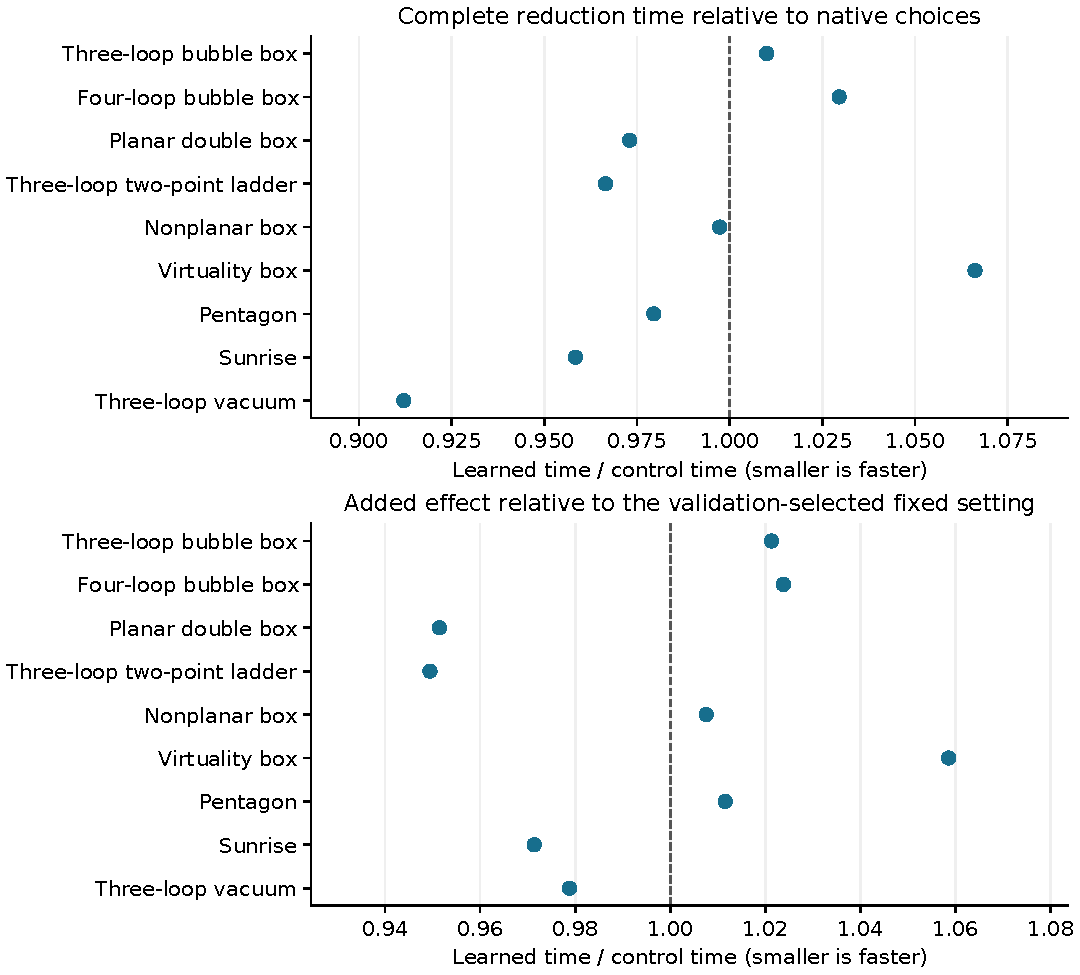
\includegraphics[width=\linewidth]{paper_figures/adaptive_reduction.pdf}
\caption{The upper panel compares the learned policy with native choices after the common exact improvements. The lower panel compares it with the best fixed validation choice. Each point divides sums of batch medians within one graph structure. Values below one indicate less time; the equal-time line remains visible. Three repetitions support descriptive comparisons, rather than a general speed guarantee.}
\label{fig:adaptive}\end{figure}

\subsection{A stronger fixed control and the deployed policy}
One fixed setting for all graphs can be a weak control because different denominator structures can favour different seed regions. We therefore select a separate fixed setting for each graph using validation data only. We also fit 21 small regression trees separately for the graphs with sufficient training cases. They use the same measured cost labels and can specialize in the effect of target powers and numerator rank within one denominator structure. Validation compares these trees with the global model and selects a predictor and gate for each graph. Fitting the additional trees takes 0.723 seconds, with no additional label-generation cost.

We compare the graph-specific fixed settings, the original global model, and a validated policy that uses its selected predictor only where validation supports an additional saving. This procedure was specified before any reserved timings were collected. The final rule requires at least two percent less summed validation time and a saving in both validation repetitions; otherwise the graph's fixed setting is used. All choices remain fixed during the matched comparison. Appendix~\ref{app:adaptive} defines the local models and selection rule.

Validation enables target-dependent predictions for planar double box, three-loop two-point ladder, nonplanar box. Table~\ref{tab:adaptive-graph} gives a separate matched comparison on the same reserved targets, with three repetitions per method. The graph-specific fixed choices take 105.909 seconds, the cost model takes 103.896 seconds, and the validated policy takes 103.983 seconds, using sums of batch medians. The validated policy uses 1.8\% less time than the graph-specific control. Across all repetitions, its time ratio is 0.9830. All 234 reductions pass exact coefficient checks. The fixed choices and validated policy require 21 and 9 recovery attempts, respectively. Figure~\ref{fig:adaptive-graph} shows where predictions add value beyond a fixed choice for each graph.

\begin{table}[!htbp]\centering\small
\caption{Matched complete times in seconds against the stronger fixed control. The validated policy keeps fixed choices where validation does not support the model.}
\label{tab:adaptive-graph}
\begin{tabular}{@{}lrrr@{}}\toprule
Graph & Fixed per graph & Cost model & Validated policy\\\midrule
Three-loop bubble box & 2.197 & 2.190 & 2.201\\
Four-loop bubble box & 28.777 & 29.170 & 28.961\\
Planar double box & 9.932 & 9.275 & 9.333\\
Three-loop two-point ladder & 23.542 & 22.620 & 22.518\\
Nonplanar box & 30.572 & 29.734 & 29.839\\
Virtuality box & 2.207 & 2.160 & 2.213\\
Pentagon & 3.124 & 3.295 & 3.371\\
Sunrise & 1.855 & 1.873 & 1.791\\
Three-loop vacuum & 3.702 & 3.576 & 3.756\\
\midrule Total & 105.909 & 103.896 & 103.983\\\bottomrule
\end{tabular}\end{table}

\begin{figure}[tbp]\centering
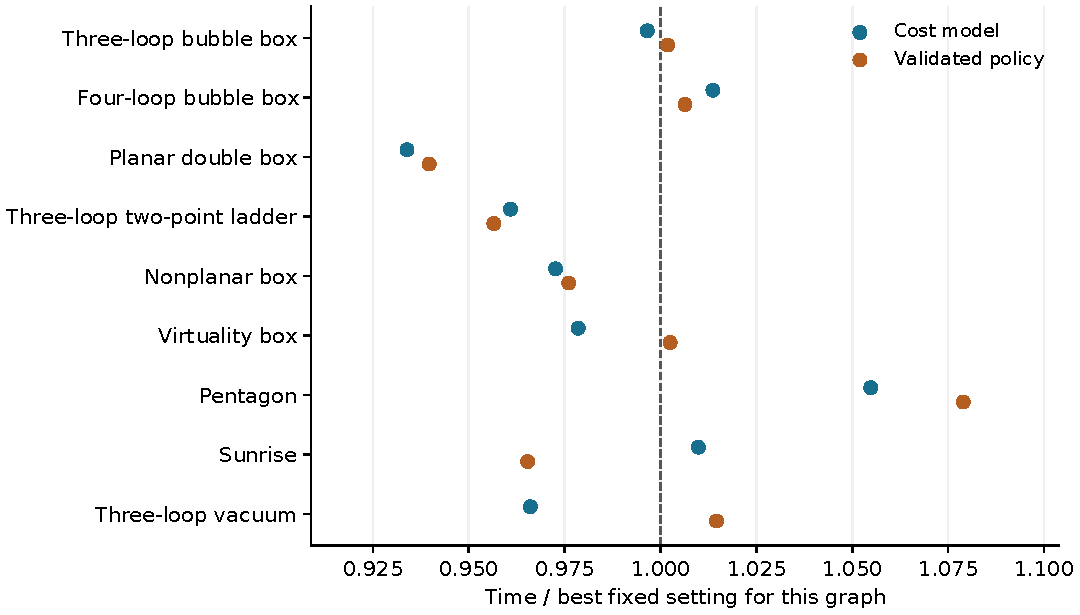
\includegraphics[width=\linewidth]{paper_figures/adaptive_graph_controls.pdf}
\caption{Added effect of target-dependent choices relative to the best fixed validation setting for each graph. Each point divides summed batch medians in the matched comparison. The validated policy uses the model only in the graph structures selected by its validation rule. Timing differences also remain when two methods choose the same setting.}
\label{fig:adaptive-graph}\end{figure}

The public application uses the validated policy and completes the separate exact checks reported above. It keeps native choices for requests outside the recorded family structures and target ranges. An additional application check confirms this fallback for an unsupported graph label. This guard limits the domain in which the learned prediction is used; it does not establish performance on unseen graph structures.

\subsection{Separating preprocessing and prediction}
We repeat the connected three- and four-loop bubble-box calculations with each exact change enabled in turn, followed by the validated policy. Table~\ref{tab:adaptive-integration} reports matched complete times from these separate trials. Every method receives the same 600-second allowance per attempt. The previous-preparation control retains declared-sector initialization and uses native equation choices in the same executable. It disables the two new exact changes. Thus the overall factor includes deterministic preprocessing as well as any subsequent benefit from its selected settings. The final change from projected preparation includes the validated policy and its graph-specific fixed settings; Figure~\ref{fig:adaptive-integration} keeps these contributions separate.

The 4-loop previous control does not complete within its bounded attempts, after 1190.6 seconds of recorded work. Its remaining 2 repetitions are omitted after this failure, while the other pre-specified settings are completed. It receives no median completion time or speedup factor.

\begin{table}[!htbp]\centering\small
\caption{Matched preparation comparison for the connected bubble boxes. Times are medians of three complete reductions, in seconds. The final column divides previous-preparation time by validated-policy time.}
\label{tab:adaptive-integration}
\begin{tabular}{@{}rrrrrr@{}}\toprule
Loops & Previous & File index & Projection & Validated policy & Overall factor\\\midrule
3 & 6.087 & 5.525 & 2.906 & 2.939 & 2.07\\
4 & Incomplete & 98.408 & 28.197 & 28.666 & --\\
\bottomrule\end{tabular}\end{table}

\begin{figure}[tbp]\centering
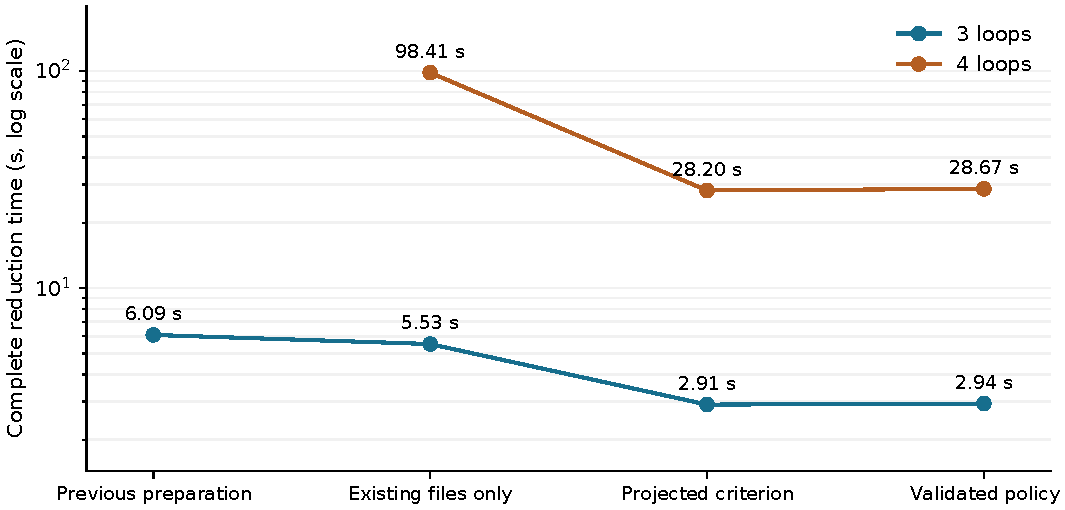
\includegraphics[width=\linewidth]{paper_figures/adaptive_integration.pdf}
\caption{Complete time for the matched preparation study. The logarithmic vertical axis displays the large deterministic change and the final change from the validated policy. The separate graph-specific comparison measures the added effect of prediction. All plotted points represent completed reductions into the same prescribed basis with exact coefficient checks. Incomplete controls are omitted from the curve and reported in the table.}
\label{fig:adaptive-integration}\end{figure}

The new policy makes one inexpensive decision before the costly work begins and retains native row elimination. Its tests cover stated target patterns and kinematics in known families. They do not establish a gain for every integral type, a minimal master basis, or a globally fastest reduction sequence. Reference failures and bounded higher-loop attempts remain part of the evidence. These limits determine where the current measurements support use of the method.
